% !TEX TS-program = XeLaTeX
% use the following command:
% all document files must be coded in UTF-8
\documentclass[english]{textolivre}
% build HTML with: make4ht -e build.lua -c textolivre.cfg -x -u article "fn-in,svg,pic-align"
\journalname{Texto Livre}
\thevolume{19}
%\thenumber{1} % old template
\theyear{2026}
\receiveddate{\DTMdisplaydate{2025}{2}{7}{-1}} % YYYY MM DD
\accepteddate{\DTMdisplaydate{2025}{5}{27}{-1}}
\publisheddate{\DTMdisplaydate{2026}{1}{21}{-1}}
\corrauthor{Vítor Hugo Barbosa dos Santos}
\articledoi{10.1590/1983-3652.2026.51173}
%\articleid{NNNN} % if the article ID is not the last 5 numbers of its DOI, provide it using \articleid{} commmand 
% list of available sesscions in the journal: articles, dossier, reports, essays, reviews, interviews, editorial
\articlesessionname{articles}
\runningauthor{Costa \textit{et al.}}
%\editorname{Leonardo Araújo} % old template
\sectioneditorname{Daniervelin Pereira~\orcid{0000-0003-1861-3609}}
\layouteditorname{Leonardo Araujo~\orcid{0000-0003-3884-2177}}

\title{Exploiting semantic similarities applied to recommender systems with Content-Based Filtering}
\othertitle{Explorando similaridades semânticas aplicadas a sistemas de recomendação com Filtragem Baseada em Conteúdo}
%\othertitle{Article template for submitting to the Texto Livre Journal}
% if there is a third language title, add here:
%\othertitle{Artikelvorlage zur Einreichung beim Texto Livre Journal}

\author[1]{Gabriel Gonçalves Faria Costa\orcid{0009-0001-3824-3441}\thanks{Email: \href{mailto:ggcosta@ufba.br}{ggcosta@ufba.br}}}

\author[1]{Diego Correa da Silva\orcid{0000-0001-7132-1977}\thanks{Email: \href{mailto:diego.correa@ufba.br}{diego.correa@ufba.br}}}

\author[1]{Guilherme Souza Brandão\orcid{0000-0002-7217-0231}\thanks{Email:\href{mailto:guilhermebrandao@ufba.br}{guilhermebrandao@ufba.br}}}

\author[1]{Vítor Hugo Barbosa dos Santos\orcid{0000-0002-1771-2624}\thanks{Email: \href{mailto:vitorbarbosa@ufba.br}{vitorbarbosa@ufba.br}}}

\author[1]{Frederico Araújo Durão\orcid{0000-0002-7766-6666}\thanks{Email: \href{mailto:fdurao@ufba.br}{fdurao@ufba.br}}}

\affil[1]{Universidade Federal da Bahia, Salvador, BA, Brasil.}

%\usepackage{biblatex}
\addbibresource{article.bib}



% use biber instead of bibtex
% $ biber article

% used to create dummy text for the template file
\definecolor{dark-gray}{gray}{0.35} % color used to display dummy texts
\usepackage{lipsum}
\SetLipsumParListSurrounders{\colorlet{oldcolor}{.}\color{dark-gray}}{\color{oldcolor}}


\usepackage{graphicx}
\usepackage{graphics}
\usepackage{algorithm}
\usepackage{algpseudocode}
\usepackage[utf8]{inputenc}


% if you use multirows in a table, include the multirow package
\usepackage{multirow}

% provides sidewaysfigure environment
\usepackage{rotating}

% used here only to provide the XeLaTeX and BibTeX logos
\usepackage{hologo}

% if you use multirows in a table, include the multirow package
\usepackage{multirow}
\usepackage{color,soul}

% provides sidewaysfigure environment
\usepackage{rotating}

% CUSTOM EPIGRAPH - BEGIN 
%%% https://tex.stackexchange.com/questions/193178/specific-epigraph-style
\usepackage{epigraph}
\renewcommand\textflush{flushright}
\makeatletter
\newlength\epitextskip
\pretocmd{\@epitext}{\em}{}{}
\apptocmd{\@epitext}{\em}{}{}
\patchcmd{\epigraph}{\@epitext{#1}\\}{\@epitext{#1}\\[\epitextskip]}{}{}
\makeatother
\setlength\epigraphrule{0pt}
\setlength\epitextskip{0.5ex}
\setlength\epigraphwidth{.7\textwidth}
% CUSTOM EPIGRAPH - END


% add line numbers for submission
%\usepackage{lineno}
%\linenumbers

\begin{document}
\maketitle
\begin{polyabstract}
\begin{english}
\begin{abstract}
The present work aimed to develop and evaluate alternative methods for similarity calculation, combining conventional approaches such as cosine similarity with the Wu-Palmer similarity, integrated into WordNet's semantic network, to improve the quality of recommendations in Content-Based Filtering recommender systems. The MovieLens small movie database and Google Collaboratory's Python programming environment were used for this. The results of the experiments indicate that Content-Based Filtering can be improved by implementing methods that leverage semantic similarity measures. In addition, the best-performing similarity measure was Wu-Palmer, as measured by Mean Reciprocal Rank and Mean Average Precision. Specifically regarding Mean Reciprocal Rank, Wu-Palmer's similarity consistently got better results through all positions, with the maximum average outperforming others. Concerning Mean Reciprocal Rank outcomes, the algorithm developed based on Wu-Palmer similarity also demonstrated the best overall performance in the experiment, achieving a maximum Mean Reciprocal Rank of 0.67 at position ten.


\keywords{Semantic similarity \sep Recommender systems \sep Content-Based Filtering}
\end{abstract}
\end{english}

\begin{portuguese}
\begin{abstract}
O presente trabalho teve como objetivo desenvolver e avaliar métodos alternativos de cálculo de similaridade, combinando abordagens convencionais, como a similaridade do cosseno, com a medida semântica de Wu-Palmer, integrada à estrutura de rede semântica WordNet, visando aprimorar a qualidade das recomendações em sistemas de recomendação baseados em Filtragem Baseada em Conteúdo. Para a condução dos experimentos, utilizou-se o conjunto de dados de curtas-metragens do MovieLens, bem como o ambiente de programação Python, executado na plataforma Google Colaboratory. Os resultados experimentais indicam que a Filtragem Baseada em Conteúdo pode ser significativamente aprimorada por meio da incorporação de medidas de similaridade semântica. Entre as abordagens avaliadas, a similaridade Wu-Palmer apresentou o melhor desempenho tanto na métrica de Classificação Recíproca Média (MRR) quanto na Precisão Média. Em particular, no que se refere à Classificação Recíproca Média, a medida de Wu-Palmer obteve resultados consistentemente superiores em todas as posições analisadas, alcançando a maior média entre as demais abordagens. De forma semelhante, na avaliação da Precisão Média, o algoritmo baseado na similaridade Wu-Palmer destacou-se pelo melhor desempenho geral, atingindo um Rank Recíproco Médio máximo de 0,67 na posição 10.

\keywords{Similaridade semântica \sep Sistemas de recomendação \sep Filtragem Baseada em Conteúdo}
\end{abstract}
\end{portuguese}

\end{polyabstract}
\section{Introduction}

%Sugestao de Ramon:

% \begin{enumerate}
%     \item contexto
%     \item qual é o problema?
%     \item por que é importante?
%     \item o que tem na literatura
%     \item qual é a lacuna/deficiência na literatura/em que as abordagens falham
%     \item qual é a nossa proposta/contribuição
%     \item resultados e principais conclusões
% \end{enumerate}

%%Context
Recommender Systems (RS) are software that present new products to consumers as recommendations. These suggestions should be personalized according to the user's preferences. RSs serve two functions: encouraging users to consume specific content or products and managing information overload. The latter often occurs when many items are available in the catalog, which might hinder user experience \cite{livro}.

The system must develop and maintain a model or profile representing user preferences to define personalized recommendations. Collaborative Filtering (CF) and Content-Based Filtering (CBF) are commonly used approaches. CF relies on historical user-item interaction data to identify user similarities and make recommendations. CBF focuses on analyzing the attributes or features of items and recommends items based on user preferences or profiles. CBF has two advantages over CF: no user group is required to make personalized recommendations, and it is robust to the cold-start problem \cite{anwar2021comparative, thorat2015survey}.

%The problem
Despite its advantages, CBF does not consistently outperform CF. This limitation stems from the inherent challenge of defining item similarity in CBF. Text as title, description, and genre, called metadata, is a common feature used to determine the similarity of the items, usually in natural language. So, choosing the correct natural language text similarity method is necessary to measure its similarity.


%Why is important
To improve CBF results, it is crucial to develop alternative methods that account for these semantic relationships to augment the precision. One potential approach is to leverage external resources, such as reference databases, or to utilize named entity recognition techniques, which identify elements in a text that correspond to real-world entities (e.g., proper nouns) and can provide insights into the content of the text in which they occur.

%What exists in the literature
Extensive research efforts have focused on improving CBF algorithms and models to address this issue \cite{wijewickrema2019selecting, oppermann2020vizcommender}. Exploring different similarity methods has shown promise in enhancing these models and algorithms. 

% Which part is not already solved
When text is the primary descriptor of an item, existing methods for calculating textual similarity often neglect the semantic relationships among keywords, making text-based comparisons difficult.


%proposed solution
This study is dedicated to enhancing CBF in RS by exploring alternative methods for calculating item similarities, specifically leveraging semantic similarity measures. The primary objective is to demonstrate the effectiveness of Wu-Palmer semantic similarity compared to traditional cosine similarity in improving recommendation accuracy. By focusing on semantic relationships, we aim to address the inherent limitations of textual-similarity methods and improve the precision of CBF algorithms.
Our approach involves experiments using a dataset of user preferences and item attributes. We will implement the Wu-Palmer semantic similarity method alongside cosine similarity and evaluate their performance using metrics such as Mean Average Precision (MAP). By comparing the recommendations generated by these methods, we aim to validate the hypothesis that semantic similarity improves the quality of item recommendations in CBF. The experiments showed that Wu-Palmer semantic similarity is more effective than cosine similarity. This means that considering semantic relationships between words yielded better comparisons between two vectors containing different words with similar meanings. Although the initial Mean Average Precision (MAP) values for all tested algorithms were low, achieving a precision above 10\% improved the recommendation ranking compared to a random selection of films.




\section{Content Based Systems} 

Over the last few years, RSs have been a valuable means of addressing information overload. However, other reasons item providers and recommender system owners might want to explore RSs include increasing the number of items sold, selling a more diverse set of items, or increasing user satisfaction and loyalty \cite{ricci}.

The RSs are software tools or techniques that suggest items likely to interest a specific user. Suggestions are usually related to various decision-making processes, such as what to buy, what to listen to, or what to watch. A CBF uses user-item interactions, such as ratings, \cite{ricci}.

Personalized recommendations are sorted lists of items that reflect user preferences and restrictions. CBF Systems collects user items to predict the most suitable items obtained from explicit similarities between them. This similarity is usually calculated using measures such as the cosine or Jaccard similarity \cite{pazzani2007content, singla2020flex}.

The CBF recommender systems have some limitations, such as limited analysis of the quality of recommended content, overspecialization, limited serendipity and diversity, issues of similarity and scalability, and inability to capture user evolution \cite{Rolim2017, javed2021review}. One of the main parts of those systems is the similarity of objects, which can be applied to items or users, usually to items. These similarities are calculated based on the features of the objects, such as text descriptions and metadata \cite{messina2019content}. That information can have high or poor quality, as it can describe the objects very well or be inaccurately represented. Also, the data can contain incorrect values, such as user data, which can introduce biases \cite{oppermann2020vizcommender}. Additionally, it is necessary to use efficient, accurate similarity methods to produce high-quality recommendations, especially when the object description is a natural-language text, such as a movie description. 


\subsection{Similarity Measures} 

A similarity measure must be used to compare items. In the present work, we compare two word vector types: the user model and a list of keywords associated with a specific movie. There are several measures, but the cosine similarity, given by \Cref{eq1}, is considered a standard metric in RSs and is also commonly used in text mining to compare documents \cite{livro}. The cosine similarity measures the angle between two n-dimensional vectors. The result is always a value between zero and one, where one represents the maximum similarity or equality between the two vectors. 

\begin{equation}
    \text{sim}( \ \overrightarrow{a} , \overrightarrow{b} \ ) = \frac{\overrightarrow{a} . \overrightarrow{b}} {\left| \ \overrightarrow{a} \ \right| * \left| \ \overrightarrow{b} \ \right|}
\label{eq1}
\end{equation}

In the present work, the cosine similarity was used. However, several other similarity measures are commonly used in recommendation systems. Two measures to be mentioned are the Pearson coefficient and the Jaccard similarity, calculated, respectively, by \Cref{eq3} and \Cref{eq4} shown below. 

\begin{equation} \label{eq3}
    \text{Pearson}(x,y) =\frac{\Sigma xy - \frac{\Sigma x \Sigma y}{N}} {\sqrt{ 
    (\Sigma x^{2} - \frac{(\Sigma x)^{2}} {N})
    (\Sigma y^{2} - \frac{(\Sigma y)^{2}} {N})
    }}
\end{equation}

\begin{equation} \label{eq4}
    \text{Jaccard}(A,B) = \frac{ \mid A \cap B \mid }{ \mid A \cup B \mid }  
\end{equation}

Pearson's Coefficient is a statistical measure that measures the degree of linear correlation between two variables, x and y. A positive correlation will produce a coefficient value greater than zero and less than or equal to 1, indicating that the two variables are directly proportional. A negative correlation, with a coefficient value less than zero and greater than or equal to minus one, indicates that the two variables are inversely proportional, in which case an increase in the value of one of the variables will produce a decrease in the value of the other. A coefficient of zero indicates the absence of any linear correlation between the two variables. 

Jaccard similarity measures the overlap between two sets and produces a value between 0 and 1. The closer to one, the more similar the two sets will be. The Jaccard coefficient is calculated by dividing the intersection of the two sets A and B, the number of elements in common between them, by the union of the two sets, and the total number of distinct elements present in the two sets A and B. 

\section{Semantic Networks and Natural Language Processing} 

Semantic networks are a type of knowledge representation that uses graphs to model concepts and their relationships. In a semantic network, concepts are represented as nodes (vertices), and their relationships are defined as edges (arcs). Nodes in a semantic network typically represent entities or concepts, such as objects, people, or ideas. The edges between nodes are predicates that represent relationships or connections between concepts. 

Semantic networks can be used for various purposes, including knowledge representation, Natural Language Processing (NLP), and information retrieval, and are particularly useful for representing complex relationships between concepts and organizing large amounts of information in a way that is easy to understand and navigate. 

A standard currently used in defining and implementing semantic networks on the web is the Resource Description Framework (RDF). RDF is used to represent interconnected data on the web. RDF instructions describe and exchange metadata, enabling standardized data exchange based on relationships among them \cite{Loshin:2022}. An RDF statement consists of three components: the subject is the resource being described; the predicate describes the relationship between the subject and object; the object is a resource related to the subject. So, in the case of the example above, the subject would be the word ``Cat'', the predicate the relation ``is a'', while the object would be the word ``Mammal''. 

Natural language means any language used for daily verbal communication between human beings. At the same time, NLP can be generically defined as any computer manipulation of a text in natural language. NLP techniques range from simple tasks, such as counting word frequencies in a text, to more complex tasks, such as interpreting its meaning. NLP is a field of artificial intelligence (AI) that aims to enable computers to interpret and generate human language. NLP involves developing algorithms and models that analyze and process text and speech data, enabling machines to perform tasks such as language translation, sentiment analysis, and question answering. NLP has widely used semantic networks to represent and process language meaning. 

One of the most well-known semantic networks used in NLP is WordNet. WordNet is a large-scale lexical database of the English language, developed by Princeton University, in which nouns, verbs, adjectives, and adverbs are grouped into sets of synonyms called ``synsets'' interconnected by semantic relationships such as hypernyms (the relationship between a general term and a more specific term) and meronymy (the relationship between a part and a whole) \cite{Fellbaum}. These ``synsets'' correspond to abstract concepts linked together in a hierarchy. More generic concepts encompass the meaning of other ``synsets'' and are called root ``synsets''. The result of this semantic network is a thesaurus that can be consulted on the Internet. 

\subsection{Semantic Similarities} 

WordNet can be used as a corpus by the Python NLTK (Natural Language Toolkit) library, thus serving as a reference for similarity calculations between semantically related words \cite{nltk}. One way to compare words using WordNet is to compare their ``lemmas''. A ``lemma'' is a generic entry in the dictionary that represents a general meaning for other words. Every word in WordNet is related to at least one ``lemma'' and this ``lemma'' can be shared between different words. From there, we can identify words with similar meanings by their ``lemmas'' in common. 

Another possible approach to word comparison is to calculate semantic similarity between terms based on their locations and potential relationships within the WordNet taxonomy. Several functions in the NLTK library can calculate semantic similarity based on the WordNet taxonomy. The method used in the present work was the Wu-Palmer similarity, as defined in \Cref{eq2}, which measures the semantic proximity between two words by considering the depth of the ``least common subsumer'' (LCS) between them. The LCS corresponds to the closest common term between two words, which is the one nearest in the WordNet hierarchy to the sum of the depths of their respective synsets, or the most specific concept that both terms share. Considering that the root depth of the WordNet taxonomy is equal to one, the LCS depth will never be zero, so the calculation result will always be a value greater than zero and less than or equal to one \cite{mohit}. 

Other similarity measures provided by the NLTK library include ``path similarity'', which returns a value between 0 and 1 representing the similarity between two synsets based on the shortest path connecting them in the WordNet hierarchy. This Leacock-Chodorow similarity returns a score based on the shortest path connecting the two meanings of the words, using the maximum depth of the taxonomy in which the meanings occur. This relationship is defined by -log(p/2d), where p is the length of the shortest path and d is the taxonomy depth. Three other similarity measures in NLTK calculate the similarity between two word meanings using the concept of ``information content'' (IC). These are the similarities of Resnik, Jiang-Conrath, and Lin \cite{nltk2023}. 

\begin{equation}
\text{WuPalmer} = 2 \ * \ \frac{depth(\ lcs(\ syn1,syn2\ )\ )}{(\ depth(\ syn1\ )\ +\ depth(\ syn2\ )\ )}
\label{eq2}
\end{equation}

The Wu-Palmer similarity measure is used in NLP and information retrieval to assess the semantic relatedness of two words in WordNet. The Wu-Palmer similarity measure calculates the relationship between two words based on their distance in the WordNet hierarchy, considering the LCS depth between the two terms \cite{wu1994palmer}. Therefore, the Wu-Palmer measure allows calculating the similarity between sets of terms that share semantic meaning, which is not possible with a non-semantic similarity measure such as the cosine. 



\section{Related Works} 

Using data from the MyAnimeList portal, \cite{zuin2016mal} developed a method to identify the central comment of a topic in a discussion forum about cartoons, avoiding the use of popularity indicators, such as likes or upvotes. As in the present work, the method involved NLP techniques with the NLTK library to map etymologically related nouns. Precision, Recall, F1 score, and MAP were used to evaluate the results. According to the article authors, the WordNet Wu-Palmer similarity was also used as an alternative, but it did not yield better results than the initial method. 

\textcite{d2017exploiting} proposes an architecture for a hybrid recommendation system that ranges from text pre-processing, using term and aspect extraction techniques, to sentiment analysis, to assign polarities to the topics evaluated by users. The text pre-processing step has some similarities wWu-Palmarethods used in the present work, such as POS tagging and the extraction of nouns that matched the main characteristics of the items. In the CF step, which was not implemented in the current work, they used the neighborhood-based recommendation algorithm. The similarity measure they used was Pearson's coefficient. The outcome evaluation measures were mean squared error, precision, and MAP. The databases were the MovieLens database, enhanced with information from the IMDB website. 

\textcite{bernardo2019cine} developed a CF recommendation system for movies using the IMDB movie database and Firebase resources. The system was designed for use on Android smartphones using Facebook login. Similarity between different users was calculated using Pearson's coefficient. The present work, however, despite being focused on movie recommendation systems, only aims to investigate other methods of calculating similarities, comparing cosine and Wu-Palmer similarities approaches in a content-filtering context. 

\textcite{almeida2020sistemas} used feature extraction techniques, Word2Vec, and TF-IDF, not used in the current project, to transform textual information related to movies into numerical values for content-based analysis. For this, a larger version, MovieLens 1M, was used, and the same dataset was used in the current project. However, for user profile learning, based on the ratings of watched movies, machine learning techniques were used to build a regression model that represents user preferences. The cosine similarity measure was used, and the evaluation metrics were Precision, Recall, Novelty, and Diversity. 

\textcite{silvasistema} developed a hybrid recommendation system for movies, combining collaborative and CBF, using contextual pre-filtering and the KNN (K-Nearest Neighbors) algorithm for CF, and the evaluative measures of Mean Absolute Error, Mean Squared Error, and Square Root of the Average Error. The database used was the same as in the present work: the MovieLens small dataset. Similarly, the movie genre attribute was used for the CBF step. However, the similarity measure implemented was the Jaccard index, not the cosine or Wu-Palmer similarity. The results indicated pure CF was better than hybrid and Content-Based approaches. 

In \cite{pradeep2020content}, a movie recommendation system was built based on cast, keywords, crew, and genre attributes. These four attributes were aggregated into a single column, creating a new attribute that served as the basis for the system. The recommendation was then made, using the cosine similarity, of another ten films similar to the first film, informed by the user. Similarly, in the current project, we concatenated each film's title, genre, and tags into a single string, from which we extracted all nouns. However, this new string of nouns served as a base attribute for creating the user model and for later comparing it with other movies. 

Using the MovieLens database, \textcite{azambuja2021teoria} presents a five-layer MLP architecture as an example of a neuronal CF model using the Jaccard coefficient as a similarity measure. The output of the proposed model consists of the ``successful percentage of movie recommendation'' for the Top N recommendations from the predictions list for each user. On the other hand, in the present content-based work, which does not employ a machine learning model or the Jaccard similarity, the final result is a ranking of the ten films most similar to the user model for each base user. The authors used precision, recall, accuracy, and F-score as evaluation metrics. In addition, they also denote the differences and complementarities between sequential recommendations, which use chronologically ordered user information, and recommendations based on sections, neither of which is considered in this work. 

The work of \textcite{silva2021uso} aimed to compare different AutoML tools applied to recommendation systems using the MovieLens database. The strategy the author addressed was CF to predict the next item the user would consume, in this case, the next movie the user would watch. Unlike the current approach, which identifies possible items that match the user's profile rather than those consumed over a given period. In the author's experiments, none of the techniques implemented by the autoML tools produced significant results. 

The research conducted by \textcite{wang2020measurement} on textual similarity measurement techniques provides fundamental insights relevant to this study. The authors comprehensively review several methods, including distance-based metrics such as cosine similarity and Jaccard index, as well as deep learning approaches such as neural embeddings. These methodologies are crucial for effectively calculating item similarity in content-based recommender systems, which aligns with the integration of the Wu-Palmer similarity measure within the WordNet semantic framework in this study. By examining applications in information retrieval and recommender systems, the study emphasizes the importance of selecting robust similarity metrics to enhance recommendation quality.
The journal by \textcite{han2021survey} on semantic similarity techniques for short texts is directly relevant to this study's focus on improving similarity measures in recommender systems. The authors explore vector-based methods, neural network architectures, and embedding models, aligning with the use of Wu-Palmer similarity within the WordNet framework in this study. By evaluating performance metrics such as Mean Reciprocal Rank (MRR) and discussing practical applications in sentiment analysis and recommender systems, their findings support the methodology of integrating advanced semantic techniques to improve the quality and relevance of recommendations. \textcite{rathee2022analysis} provides an analysis of semantic similarity measures in information retrieval, offering a detailed examination of metrics such as WordNet-based similarity and neural embeddings, directly applicable to this study's focus on improving content-based filtering. The authors evaluate criteria such as precision and computational efficiency, offering insights into selecting effective similarity measures. By discussing applications in document clustering and recommender systems, their findings highlight the relevance of this study's approach to integrating the Wu-Palmer similarity to optimize recommendation quality. The study by \textcite{chandrasekaran2021evolution} on the evolution of semantic similarity techniques offers insights into advanced methodologies that inform this study. The authors trace the progression from traditional methods to modern approaches that utilize embeddings and neural networks, which are fundamental to understanding how semantic relationships impact recommender systems. This evolution aligns with the exploration of Wu-Palmer similarity integration within the WordNet framework in this study, highlighting the importance of leveraging semantic context to improve recommendation accuracy. Its comparative analysis in natural language processing and recommender systems provides a theoretical framework that validates the focus on improving content-based filtering through semantic enhancements.



\section{Exploring semantic similarities applied to recommender systems with Content-Based Filtering} 

The present work aims to investigate alternative methods for calculating similarity in recommendation systems using CBF. More specifically, where it is necessary to compare two keyword lists or vectors: one that describes a user´s movie preferences and another that refers to a movie´s characteristics. For this, the performances of four different similarity calculation methods, as described in \Cref{recommendation-model}, were compared. Of the four implemented methods, one uses the Wu-Palmer semantic similarity, and two use cosine similarity, one applied to nouns and the other to their respective lemmas according to the WordNet taxonomy. The last is a control method that uses predefined functions from the Python Scikit-learn library to calculate the cosine of the nouns.  

\subsection{Architecture} 
\label{architecture-sub}

The initial project's architecture can be divided into two essential elements. The first element consists of creating strings (vectors) containing keywords that define a movie´s characteristics, generated from its title, genre, and any user tags associated with the movie. Having generated the strings for all movies, they are kept in memory as a movie attribute to define user models and subsequent recommendations. 

NLP techniques were used to extract the relevant terms from the title and genre attributes and the movie tag table, which were included in the respective keyword vectors or movie strings. For the present work, the Python library NLTK was used to implement the necessary NLP techniques \cite{nltk}. The first technique implemented was the ``tokenization'' of text strings. Tokenization is the process of splitting a sentence or a string of words into a list of its constituent elements. Once the list is generated by tokenizing the string, the next step is called ``part-of-speech tagging'' (POS-tagging). 

During POS tagging, each term in the list produced by the tokenization process receives a label indicating its part of speech. That label informs whether that term is a noun, verb, adjective, or other word class. The result of POS-tagging is a list of tuples containing the term plus its grammatical label. From there, words belonging to a specific grammatical category can be easily filtered from the source text. For example, to extract all nouns, one only needs to search the list of tuples for terms with labels corresponding to the different types of identified nouns: `NN' for singular nouns; `NNS' for plural nouns; `NNP' or `NNPS', respectively for singular and plural proper nouns. \Cref{fig:moviestring} presents the processes involved in this first stage. 

\begin{figure}[hbt!]
\centering
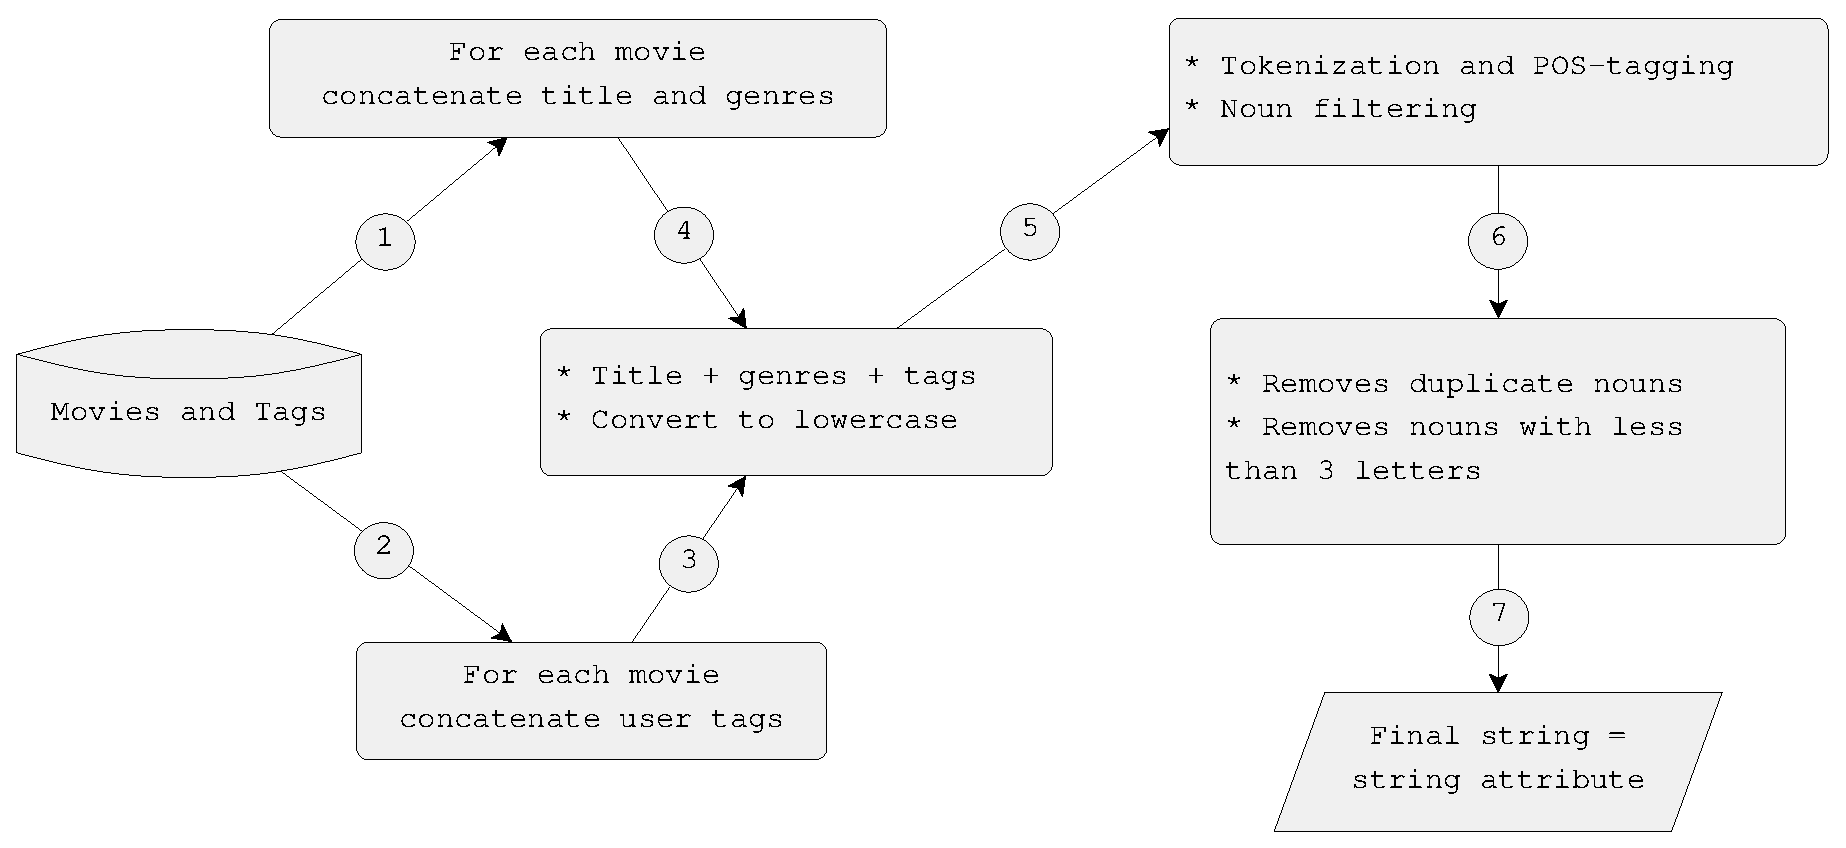
\includegraphics[width=\textwidth]{diagramas/fig-003.eps}
\caption{Process of creating the movie strings.}
\label{fig:moviestring}
\source{Own elaboration.}
\end{figure}

Initially, the film titles and their respective genres are concatenated (arrow 1). In contrast, the user tags for the respective movie are concatenated separately (arrow 2). The two strings are united into a single string, and all the capital letters of the resulting string are converted to lowercase (arrows 3 and 4). Tokenization followed by POS-tagging of this exact string generates a list of tuples containing words with their respective grammatical classes, from which all nouns are filtered (arrow 5). Duplicate nouns and those with fewer than three letters (arrow 6) are removed. From the resulting list of distinct nouns with more than three letters, the film's new ``string'' attribute is constituted (arrow 7). 

The second element consists of defining the user model, which, in this case, corresponds to a list of the most frequently associated words with the user's best-rated movies, presumably related to the user's preferences. \Cref{fig:usermodel} shows the process of defining the user model from the movie strings. 

\begin{figure}[hbt!]
\centering 
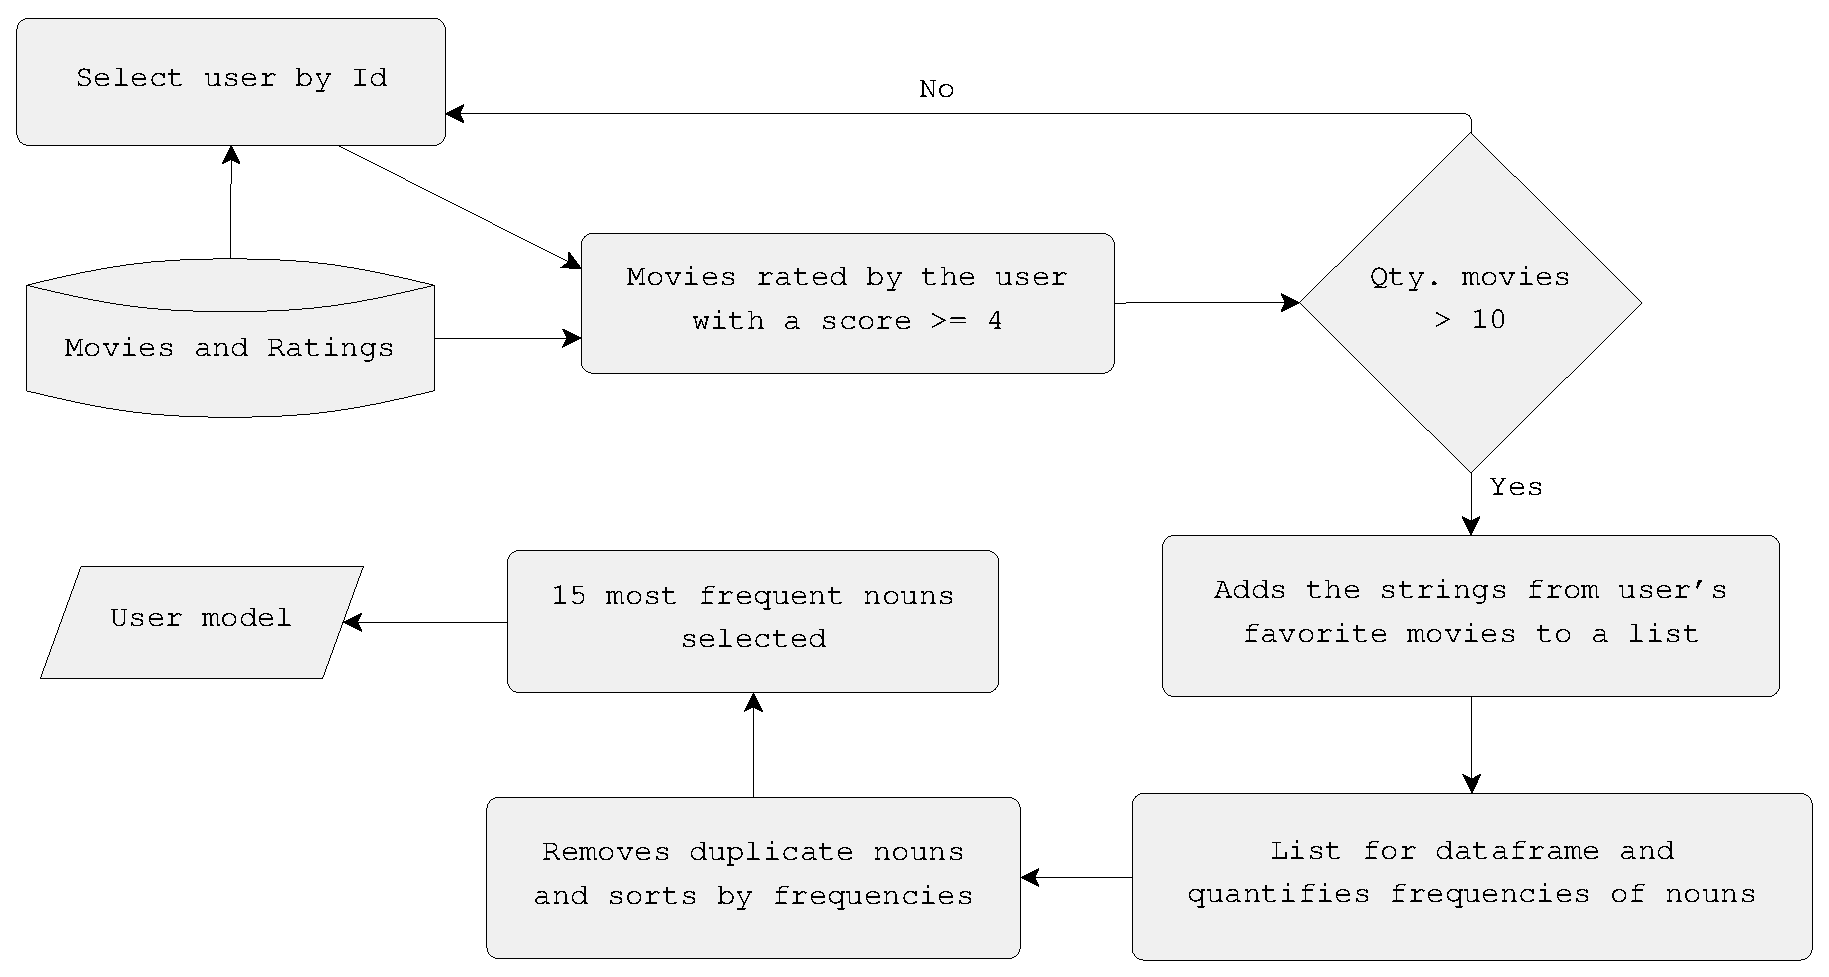
\includegraphics[width=\textwidth]{diagramas/fig-004.eps}
\caption{User model creation process.}
\label{fig:usermodel}
\source{Own elaboration.}
\end{figure}

From the user ID, all movie IDs rated by the user with a score of 4 or higher are extracted from the rating file. A new user must be selected if the user has evaluated fewer than 10 films. Once all movie IDs have been collected, their respective strings are concatenated into a single list of nouns. This list is converted to a data frame, and the frequencies of equal nouns are quantified and ordered from highest to lowest. The fifteen most frequent distinct nouns are selected for the user model. 

\subsection{Recommendation model} 
\label{recommendation-model}

The recommendation process consists of comparing a user model with a movie string. To do so, any number of films the user has not yet evaluated can be drawn. Each film is compared individually with the user model. Afterward, all drawn films are ordered by similarity. The N films at the top of the list with the most significant similarity can be presented as recommendations. \Cref{fig:comparison} generally shows how the comparison process works. 

\begin{figure}[hbt!] \centering
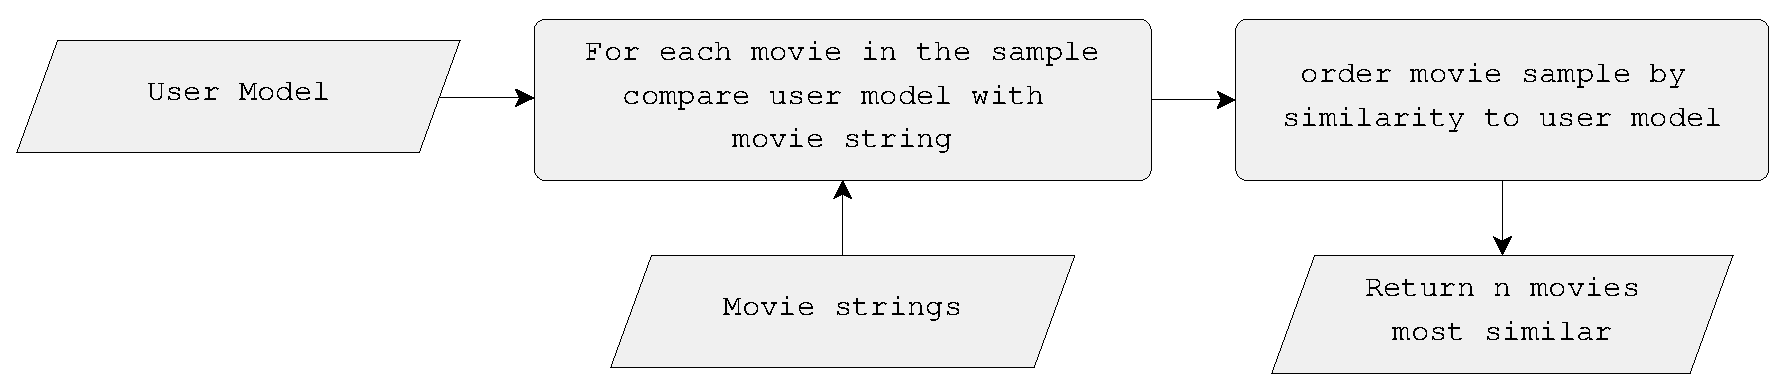
\includegraphics[width=\textwidth]{diagramas/fig-005.eps} 
\caption{Comparison between user model and movie string.} 
\label{fig:comparison} 
\end{figure} 

Four different methods of comparison by similarity measures were evaluated. The Wu-Palmer maximums' average method, as presented in the Algorithm pseudocode \Cref{alg:1}, finds the maximum Wu-Palmer similarity for each of the user model´s nouns with respect to all the nouns in the movie string. The highest recorded value is stored in a list, and the mean of these maximum similarities is then calculated. 

\begin{algorithm}[hbt!]
\caption{Averaging the Wu-Palmer maximums.}\label{alg:1}        
    {\small
    \begin{algorithmic}[1]
    \State Takes two lists of nouns: $list0$, $list1$
    \State Initialize list $values$
    \State Initialize list $maximums$ list
    \State Initialize $aux$ = 0
    \For {each $noun$ in $list0$}
        \State $synset0$ = $noun$ synset in WordNet
        \If {$length(synset0) > 0$}
            \State clear list $values$
            \For{each $noun$ in $list1$}
                \State $synset1$ = $noun$ synset in WordNet
                \If{$length(synset1) > 0$}
                    \State $aux$ = wu-palmer similarity between $synset0[0]$ and $synset1[0]$
                    \If{$aux == 1$}
                        \State\textbf{break}, max value for $synset0$ found 
                    \Else
                        \State Adds $aux$ to list $values$ 
                    \EndIf
                \EndIf
            \EndFor
            \If{$aux == 1$}
                \State Adds $aux$ to $maximums$ 
            \Else
                \State Adds maximum of $values$ to $maximums$
            \EndIf
        \EndIf
    \EndFor
    \If{$length(maximums) == 0$}
        \State\textbf{Return} $None$ 
    \Else
        \State \textbf{Return} $sum(maximums)/length(maximums)$ 
    \EndIf
    \end{algorithmic} 
    } 
\end{algorithm} 

To illustrate how the Wu-Palmer maximum averaging works, we can consider the two-word vectors: A = [``cat'', ``dog''] and B = [``wolf'', ``bear'']. Firstly, we calculate the Wu-Palmer similarities of all combinations of terms between the two vectors and select the most considerable result for each term for one of the vectors. Considering vector A, the most significant similarity for the first term of the vector is with the second term of vector B. That is, between the two-word combinations cat " +" wolf" and cat " + "bear," the second combination yields the highest similarity value, approximately 0.89. The second term's highest similarity corresponds to the pair dog " + "wolf'', with approximately 0.93. Then we calculate the arithmetic mean of these two values, yielding a similarity of roughly 0.91 between the two vectors. This implementation of the Wu-Palmer maximums' average will always generate values greater than zero and less than or equal to one. The maximum value of one is obtained when two similar vectors are compared, containing the same terms regardless of the order in which they occur inside the vectors. 

The cosine method, based in part on the online material by \cite{Puri:2018}, considers only the single occurrences of terms in two-word lists or vectors. First, the two term lists are converted into data frames with a single frequency column. Then, the union, or a \emph{merge}, of the two data frames is performed as exemplified in \Cref{table:1}. A third data frame is generated, containing all the terms of both data frames plus two columns, one for each original list of terms, indicating whether the term occurs in the respective list. This union of two data frames computes the cosine similarity between the two lists of terms using the pseudocode for Algorithm \Cref{alg:2}. 

\begin{table}[hbt!]
\centering
\caption{\emph{Merge} between two tables of terms and frequencies.}
\label{table:1}
%\renewcommand{\arraystretch}{1.2} % Default value: 1
    {%\footnotesize
    \begin{tabular}{c c} 
        \toprule
        Term & $freq_x$ \\ 
        \midrule
        airbnb & 1.0\\
        china & 1.0\\
        country & 1.0\\
        listings & 1.0\\
        lockdowns & 1.0 \\
        years & 1.0 \\
        \bottomrule
    \end{tabular}
    \hfill + \hfill
    \begin{tabular}{cc} 
        \toprule
        Term & $freq_y$ \\ 
        \midrule
        airbnb & 1.0 \\
        china & 1.0 \\
        experiences & 1.0 \\
        listings & 1.0 \\
        offers & 1.0 \\ 
        summer & 1.0 \\
        \bottomrule
    \end{tabular}
    \vspace{10pt}
    \hfill = \hfill
    \begin{tabular}{ccc} 
        \toprule
        Term & $freq_x$ & $freq_y$ \\ 
        \midrule
        airbnb & 1.0 & 1.0 \\
        china & 1.0 & 1.0 \\
        country & 1.0 & 0.0 \\
        experiences & 0.0 & 1.0 \\
        listings & 1.0 & 1.0 \\
        lockdowns & 1.0 & 0.0 \\
        offers & 0.0 & 1.0 \\ 
        summer & 0.0 & 1.0 \\
        years & 1.0 & 0.0 \\
        \bottomrule
    \end{tabular}
    }
\source{Own elaboration.}
\end{table}

\begin{algorithm}[hbt!]
\caption{Cosine similarity calculation.}\label{alg:2} 
    {\small
    \begin{algorithmic}[1]
    \State Takes two lists of nouns: $list0$, $list1$
    \State Convert $list0$ to $df0$ with frequency column
    \State Convert $list1$ to $df1$ with frequency column
    \State Merge of $df0$ and $df1$ produces data frame $mergedf$ with frequency columns $\text{freq}_x$ and $\text{freq}_y$ corresponding to the occurrence of each term in both lists.
    \end{algorithmic}
    \begin{algorithmic}[1]
    \For{each line in mergedf}
        \State $\text{numerator} += \text{row}[\text{freq}_x] * \text{row}[\text{freq}_y]$
        \State $\text{vector}_x += \text{line}[\text{freq}_x]^2$
        \State $\text{vector}_y += \text{line}[\text{freq}_y]^2$ 
    \EndFor
    \State $\text{denominator} =\sqrt{\text{vector}_x} *\sqrt{\text{vector}_y}$
    \State\textbf{return} $\text{numerator}/\text{denominator}$
    \end{algorithmic} 
    } 
\end{algorithm} 

The cosine similarity method is used to compare nouns and their lemmas. For the second method, the lemmas of the respective nouns of the two strings to be compared must first be extracted from WordNet. The Algorithm Pseudocode \Cref{alg:3} represents the process by which lemmas are found for a given vector of nouns. First, the noun´s synset is checked, after which the synset´s respective lemma is checked. The last evaluated method was a control method, used to compare with the first three, which used predefined functions from the Scikit-learn library \cite{scikit-learn} to calculate cosine similarity between nouns. 

\begin{algorithm}[hbt!]
\caption{Extraction of lemmas from nouns.}\label{alg:3}
    {\small
    \begin{algorithmic}[1]
    \State Get list $nouns$
    \State Initialize list $lemmas$
    \For{each $noun$ in $nouns$}
        \State $synset$ = $noun$ synset in WordNet
        \If {$length(synset) > 0$}
            \If{$length(lemmas(synset[0])) > 0$}
                \State Adds the first lemma of $synset[0]$ to $lemmas$ 
            \EndIf
        \EndIf
    \EndFor
    \State \textbf{Return} $lemmas$ dataframe
    \end{algorithmic} 
    } 
\end{algorithm} 

\subsection{Recommendation in action} 

A recommendation scenario with three random movies not rated for a given user can occur as follows. The survey of well-evaluated films, with grades between 4 and 5, by the user of Id = 1 produced the following user model: \emph{“action-adventure comedy-drama thriller crime children animation romance war fantasy mystery horror Disney story”}. Considering the following movie IDs and their respective strings: 32898, \emph{“trip moon voyage lune action adventure”}; 86290, \emph{“bill story comedy documentary”}; 184997, \emph{“love simon comedy-drama”}. Using the Wu-Palmer maximum average comparison method, the results in \Cref{table:2} are obtained for each film. 

\begin{table}[hbt!] 
\centering
\begin{threeparttable}
\caption{Example recommendation using Wu-Palmer based similarity measure.}\label{table:2}
    \begin{tabular}{c c} 
        \toprule
        Movie Id & Wu-Palmer maximums average\\ 
        \midrule
        184997 & 0,5693\\ 
        86290 & 0,5193\\ 
        32898 & 0,4755\\ 
        \bottomrule
    \end{tabular} 
\source{Own elaboration.}
\end{threeparttable}
\end{table} 

Based on the results of the similarity analysis, we can rank these three films for user recommendations. As shown in \Cref{table:2}, the first movie recommended is id 184997, followed by 86290, and lastly 32898. The process can be repeated using the other three similarity measures evaluated to confirm the recommendation results. For example, a new ranking is generated using the cosine similarity of the lemmas for these three films and users, as shown in \Cref{table:3}. 

\begin{table}[hbt!] 
    \centering
    \begin{threeparttable}
    \caption{Example recommendation using the cosine of WordNet lemmas.} \label{table:3} 
    \begin{tabular}{cc} 
        \toprule
        Movie Id & Cosine of lemmas\\ 
        \midrule 
        86290 & 0,2582\\ 
        184997 & 0,2582\\ 
        32898 & 0,2309\\ 
        \bottomrule
    \end{tabular} 
    \source{Own elaboration.}
    \end{threeparttable}
\end{table} 

Considering these two rankings, obtained using different similarity measures, we can conclude that the film with ID 32898 is the least suitable for recommendation, as it ranked last in both rankings. However, it would not be possible to define with certainty the most appropriate film to recommend because, although film 184997 ranked first in the ranking by first similarity, it appears tied with film 86290 in the cosine of the lemmas. But even so, if we used the first similarity as a tiebreaker, we could assume that 184997 would be the most nominated among the two remaining films. 

\section{Experimental evaluation} 

The experiment was implemented entirely in Python using Google's Collaborative Development Environment. In addition to NLTK, other Python libraries included Pandas and Numpy for data manipulation, Matplotlib for graphing the results, and Scikit-learn for controlling the cosine similarity measure. The database´s CSV files were hosted in a public GitHub repository and read in Collaboratory using Pandas library functions. 

A small MovieLens database was used to experiment. The information contained in the attributes title, genre, and tags for a specific movie was aggregated into a single list of words, from which nouns were extracted using NLP features in the Python NLTK library. The resulting list of nouns served as the basis for making the user model and calculating the similarity between the user model and specific movies. 

The methodology of this study differs significantly from the approach described in \cite{wang2020measurement} in their article "Measurement of Text Similarity: A Survey". The experiment described here was implemented in Python using Google's collaborative development environment and the NLTK, Pandas, Numpy, Matplotlib, and Scikit-learn libraries for data manipulation, visualization, and control of the cosine similarity measure.

On the other hand, \cite{wang2020measurement} focused on reviewing and categorizing text similarity measurement techniques. They reviewed vector-based methods such as TF-IDF and Word2Vec, statistical methods including cosine similarity and Jaccard, and machine learning-based methods such as neural networks and pre-trained language models. They also discussed the use of hybrid techniques that combine several approaches to improve the accuracy of similarity measurement.

In contrast, the present study used the small MovieLens database, aggregating information from the title, genre, and tags attributes into a list of words. From this list, nouns were extracted using NLP resources from the NLTK library. This list of nouns was used to create the user model and to compute the similarity between the user model and specific movies.

Uniquely, the authors provided a comprehensive theoretical view of text similarity measurement techniques, without a specific focus on practical implementation in a particular database, such as MovieLens.



\subsection{Methodology} 

The first stage of the experiment consists of loading the database files into data frames in the Collaboratory environment, followed by creating keyword vectors for each movie, as already described in the previous section, as shown in \Cref{fig:moviestring} in \Cref{architecture-sub}. The second stage comprises the sequential analysis of all 610 users registered in the database and can be divided into four other phases: 

\begin{enumerate} 
\item Defining the user model for a particular user, as depicted in \Cref{fig:usermodel} in \Cref{architecture-sub}. 

\item Draw the movie test sample using the user ID number as a seed for generating random numbers ranging from 1 to 9999, skipping existing IDs. Ten movies are drawn from among the user's favorites, and other unknown ninety movies, so the total candidate set of test movies contains one hundred movies, 90\% of which were not rated by the user and another 10\% that are part of his subset of favorites. The number of users' favorite films is not fixed. The candidate set comprises 100 movies. The successful recommendations must include 10 of the 100 films to be analyzed.


\item We repeat the previous step for each user and recommend 10 movies out of the 100 items in the candidate set. The recommendation is based on the algorithms presented in the proposal´s section. To generate the top 10 recommendations, the movies from the user profile are all compared against the 100 items in the test set.

\item The metrics MAP (Mean Average Precision) and MRR (Mean Reciprocal Ranking) @ positions 3, 5, and 10 were calculated in the last phase. The metrics are applied exclusively to the 10 items recommended.
\end{enumerate} 

 

\subsection{Data set} 

The database used in the project was the Movielens small dataset, obtained from the Grouplens website, a research group at the Department of Computer Science and Engineering at the University of Minnesota. MovieLens is a movie recommendation site with thousands of registered users \cite{grouplens}. 

The MovieLens small database contains user ratings on a scale of 1 to 5 stars and free-text tags for various movies. The database has 100.836 ratings and 3683 tags from 610 users for 9742 movies, collected between March 1996 and September 2018 \cite{movielens}. The database is divided into four files: links.csv, movies.csv, ratings.csv, and tags.csv. The links.csv file was not used in the project. The ratings.csv file contains user ratings organized by userId, movieId, rating, and timestamp attributes. Similarly, the tags.csv file includes the user tags about the movies. It has the same characteristics as userId movieId, which respectively identify the user and movie, plus the attributes tag and timestamp. For the present work, the timestamp attributes were ignored in both files. The movies.csv file contains information about movies, including movie titles and genre attributes. 

The database files were initially downloaded from the Grouplens website. Timestamp attributes have been deleted from rating files and user tags. The movies.csv, ratings.csv, and tags.csv files were then stored in a public GitHub repository, from which they were loaded into the Google Colab development environment in raw format using the Pandas library's CSV reader. 

\subsection{Evaluation metrics} 

Appropriate evaluation metrics are necessary to compare the results of the different recommendation rankings defined from the other similarity calculation methods used in the experiment. For this, two metrics based on binary ranking, where each position in the result can represent either error or success, are commonly used today. These were the MAP and MRR for all users in the database that produced results. 

The precision at the K position, or P@K, given by \Cref{eqn: P@k}, calculates the percentage of hits up to a particular position K in the ranking. For example, the precision in position three will count all hits, represented by the letter r, from the first position in the ranking to the third position, ignoring the positions below three. 

\begin{equation} 
\label{eqn: P@k} 
    P@K=\frac{r}{K} 
\end{equation} 

In this work, two P@K-based measures were used. The first measure was the average P@K, or aP@K, defined in \Cref{eqn: aP@K} as the average of all precisions at all positions up to position K for a given ranking of a user sample. For the aP@3 of any ranking generated by a given similarity measure for a single user, the arithmetic mean of all P@K precisions from position one to three of the ranking is calculated. In this context, $N = K$.

\begin{equation} 
\label{eqn: aP@K} 
    aP@K=\frac{1}{N=K}\sum_{i=1}^{N}P@K 
\end{equation} 

The second measure was the mean of the aP@Ks, or MAP, presented in \Cref{eqn: MAP}, where the means of the respective aP@Ks for all test users $U$ are calculated for each of the evaluated similarity measures at positions three, five, and ten. So, if there are N user rankings, each with its aP@3 for a given similarity measure, the MAP@3 is the mean of the aP@3 across all users. 

\begin{equation} 
\label{eqn: MAP} 
    MAP@K = \frac{1}{U}\sum_{i=1}^{U}aP@K 
\end{equation} 

The reciprocal rank (RR) is defined by the accuracy of the first hit detected, according to its respective position in the ranking. For example, in a ranking where the first hit is detected in the third position, the RR of this ranking of recommendations, represented by $N$ will be defined as 1/3 even if the final position K contemplated by the metric is below three. The last evaluation measure implemented in the work was the MRR, defined in \Cref{eqn: MRR}, which corresponds to the average of all RR obtained in the experiment for each similarity measure evaluated at positions 3, 5, and 10. 

\begin{equation} 
\label{eqn: MRR} 
    MRR@K=\frac{1}{N}\sum_{i=1}^{N}RR@K 
\end{equation} 

The MRR score ranges from 0 to 1, with higher scores indicating a better ranking algorithm. An MRR value of one means that the first relevant item is always in the top-ranking position for all queries. At the same time, a score of zero indicates that no relevant item is ever found in any position among all rankings. 

\subsection{Results} 

Complete results were obtained for 557 of the 610 database users. Of the 53 users who did not produce results, 40 did not have a sufficient number of favorite movies, rated between four and five stars, previously defined as at least greater than ten, to produce the user model. The other 13 remaining users did not produce complete results for all similarity measures and were excluded from the final results. 

 \Cref{fig:ap@k} shows the average precisions (aP@K) results for all valid users in positions three, five, and ten for each evaluated similarity calculation method, where the orange line marks the median. At the same time, the dashed green indicates the MAPs for their respective positions.
\begin{figure}[ht]
    \centering
    \begin{subfigure}{0.46\textwidth}
        \centering
        \includegraphics[width=\linewidth]{figuras/fig-006.png}
        \caption{}
    \end{subfigure}
    \hfill
    \begin{subfigure}{0.46\textwidth}
        \centering
        \includegraphics[width=\linewidth]{figuras/fig-007.png} %ap_cos_ls
        \caption{}
    \end{subfigure}
    \\
    \begin{subfigure}{0.46\textwidth}
        \centering
        \includegraphics[width=\linewidth]{figuras/fig-008.png} %ap_cos_ns
        \caption{}
    \end{subfigure}
    \hfill
    \begin{subfigure}{0.46\textwidth}
        \centering
        \includegraphics[width=\linewidth]{figuras/fig-009.png} %ap_cos_sk
        \caption{}
    \end{subfigure}
    \caption{Average precisions.}
    \label{fig:ap@k}
    \source{Own elaboration.}
\end{figure}

As shown in the graphs, the cosine of lemmas and nouns yields better-quality results than the other three measures, with significantly fewer outliers after position 10, slightly higher upper quartiles, and fewer outliers at positions 5 and 3. However, in all three measures, the medians were well below 0.2. 

The measure calculated from the Wu-Palmer maximums average showed better-quality results than the other three measures, with significantly fewer outliers in position five, no outliers detected, and a median above 0.3 at position three of the ranking. 

The results for the MAPs shown in \Cref{table:maps} indicate better precision for the similarity measure calculated from the Wu-Palmer maximum average, although they also show the most significant deviations in all three evaluated positions, followed by the cosine similarity of the nouns with the second-best performance. The lemma's cosine achieved slightly better precision at position ten when compared to the nouns' cosine using the Scikit-learn library. In comparison, the latter achieved better precision at position three and tied for fifth place with the lemmas cosine. 

\begin{table}[hbt!]
    \centering
    \caption{MAPs and standard deviations.}
    \label{table:maps}
    \renewcommand{\arraystretch}{1.2} % Default value: 1
    {\footnotesize
    \begin{tabularx}{\textwidth}{|X||>{\centering\arraybackslash}X|>{\centering\arraybackslash}X||>{\centering\arraybackslash}X|>{\centering\arraybackslash}X||>{\centering\arraybackslash}X|>{\centering\arraybackslash}X|}
        \hline
        \multicolumn{7}{| c |}{Mean Average Precisions (MAP)}\\
        \hline\hline
        Measure & MAP@3 & SD & MAP@5 & SD & MAP@10 & SD\\
        \hline
        \textbf{max\_wp} & 0.37 & 0.32 & 0.28 & 0.24 & 0.19 & 0.15\\
        cos\_ns & 0.24 & 0.28 & 0.19 & 0.21 & 0.13 & 0.13\\
        cos\_ls & 0.21 & 0.27 & 0.17 & 0.2 & 0.12 & 0.12\\
        cos\_sk & 0.22 & 0.28 & 0.17 & 0.21 & 0.11 & 0.13\\
        \hline
    \end{tabularx}
    }
    \source{Own elaboration.}
\end{table}

Looking at \Cref{fig:map2}, it is possible to notice a decreasing pattern of MAPs as there is an increase in the number of positions contemplated for all four similarity measures. The best precisions were obtained for up to the third position, while the worst ones were obtained for up to the tenth position. The deviations also presented corresponding results. In this case, the deviations were more significant for the minor positions. The highest precision was observed at positions three and five for the Wu-Palmer similarity measure. 

\begin{figure}[hbt!]
    \centering
    \begin{subfigure}{0.45\textwidth}
        \centering
        \includegraphics[width=\textwidth]{figuras/fig-010.png} %grupo-map
        \caption{}
    \end{subfigure}
    \hfill
    \begin{subfigure}{0.45\textwidth}
        \centering
        \includegraphics[width=\textwidth]{figuras/fig-011.png} %desvio-map
        \caption{}
    \end{subfigure}
    \caption{Graphs of MAPs and respective deviations.}
    \label{fig:map2}
    \source{Own elaboration.}
\end{figure}

\Cref{table:mrrs} shows the values of the MRRs and their respective deviations for the four similarity measures investigated. As in the case of MAP, the measure that performed best across all positions was based on the Wu-Palmer similarity maximums. However, the highest values were in the most prominent positions, with 0.67 and 0.66, respectively, in positions ten and five. Deviation values were also relatively low, with very close deviations at higher positions for all similarity measures. 

\begin{table}[hbt!]
    \centering
    \caption{MRRs and standard deviations.}
    \label{table:mrrs}
    \renewcommand{\arraystretch}{1.2} % Default value: 1
    {\footnotesize
    \begin{tabularx}{\textwidth}{|X||>{\centering\arraybackslash}X|>{\centering\arraybackslash}X||>{\centering\arraybackslash}X|>{\centering\arraybackslash}X||>{\centering\arraybackslash}X|>{\centering\arraybackslash}X|}
        \hline
        \multicolumn{7}{|c|}{Mean Reciprocal Ranks (MRR)} \\
        \hline\hline
        Measure & MRR@3 & SD & MRR@5 & SD & MRR@10 & SD\\
        \hline
        \textbf{max\_wp} & 0.64 & 0.43 & 0.66 & 0.39 & 0.67 & 0.38\\
        cos\_ns & 0.45 & 0.43 & 0.49 & 0.41 & 0.51 & 0.38\\
        cos\_ls & 0.42 & 0.43 & 0.45 & 0.41 & 0.48 & 0.38\\
        cos\_sk & 0.44 & 0.44 & 0.47 & 0.42 & 0.49 & 0.4\\
        \hline
    \end{tabularx}
    }
    \source{Own elaboration.}
\end{table}

As shown in \Cref{fig:mrr2}, the Wu-Palmer maximum's average yielded better MRR results across all positions than those of the other similarity measures. The standard deviations remained more or less the same, with the slightest deviations found in position ten and the largest in position three for all similarity measures investigated. 

\begin{figure}[hbt!]
    \centering
    \begin{subfigure}{0.45\textwidth}
        \centering
        \includegraphics[width=\textwidth]{figuras/fig-012.png} %grupo-mrr
        \caption{}
    \end{subfigure}
    \hfill
    \begin{subfigure}{0.45\textwidth}
        \centering
        \includegraphics[width=\textwidth]{figuras/fig-013.png} %desvio-mrr
        \caption{}
    \end{subfigure}
    \caption{Graphs of MRRs and respective deviations.}
    \label{fig:mrr2}
    \source{Own elaboration.}
\end{figure}


\subsection{Discussion} 

The experiment results indicate better performance for the algorithm based on the Wu-Palmer semantic similarity, as measured by MAP and MRR, compared with cosine-based similarity measures. However, the two metrics used yielded conflicting results about which ranking position yielded the best result. 

Considering the MAPs, the results may initially seem low across all the algorithms tested, with the highest value in position 3 for the Wu-Palmer-based similarity, at 37\% precision. This can be explained by the fact that the movie sample contains only 10\% of the user's favorite movies. Therefore, in a random ranking, the expected precision would be 10\%, i.e., the proportion of users' favorite movies in the total sample. Therefore, although low, a precision above 10\% in this case may indicate a result above that expected from a random draw of films for recommendation. This means that all tested similarity calculation methods appear to have positively affected the recommendation ranking at some position, but especially the method based on Wu-Palmer similarity at positions three and five. It is important to note that all MAPs also had significant standard deviations, meaning the recommendations would not be relevant in many cases. 

Regarding the MRR results, the algorithm developed based on the Wu-Palmer similarity also achieved the best results in the experiment, with a maximum MRR of 0.67 at position 10. Contrary to the MAP metric, the MRR standard deviation was higher when MRR was lower. For example, in the Wu-Palmer maximum average algorithm, the highest MRR value showed the least deviation among the three evaluated positions. Except for the cosine method using the Scikit-learn library, which showed the most significant deviation at position three, all other techniques showed the same tendency: lower standard deviations with larger MRRs, and all methods, without exception, presented better MRRs when counted to a greater number of positions. That is, the MRR results indicate an increase in the quality of recommendations at position ten when compared to positions five or three. 

\section{Conclusion, improvements and future work} 

This work aimed to develop and evaluate a new similarity calculation method that accounts for semantic relationships among keywords. The experiments in this study underscore the significance of incorporating semantic relationships into similarity calculations for CBF recommender systems. Specifically, our findings reveal that the Wu-Palmer semantic similarity method outperforms the traditional cosine similarity method. This improvement is crucial, as it enhances the accuracy of recommendations by better capturing the nuanced similarities between items described by different but semantically related keywords. This new method was to be used in CBF-based recommendation systems to improve the quality of the system's movie recommendations, making them more aligned with users' preferences. 

The MovieLens small database defined vectors of nouns corresponding to movies and user preferences. By comparing the movie's keyword vector with a vector representing the user model, we determined the degree of similarity between the movie and the user's preferences. The semantic similarity measure taken as the basis for our new method was the Wu-Palmer, based on the WordNet taxonomy and available through the NLTK library. Three other similarity measures were also evaluated: A simple implementation of the cosine of nouns and the cosine of lemmas according to the WordNet structure, and the cosine of nouns using native methods from the Scikit-learn library. Among the four methods tested, the one that yielded the best results for average precision and reciprocal ranking was the Wu-Palmer semantic similarity method. Therefore, we can argue that a similarity measure that accounts for semantic relationships between words can yield better results when comparing two vectors containing different words that share similar meanings. 

In the current work, only the attributes of title, genre, and user tags were used to produce the keyword vectors for the films and, consequently, the user models. A possible improvement to the current methodology would be to use additional data sources about the films in the database, such as synopses or film reviews, to enhance the films' keyword vectors. Additionally, it would be pertinent to explore integrating semantic information into cosine similarity measures via word embeddings. This aspect, not addressed in the current study, could provide valuable insights for future research efforts in enhancing recommendation systems. As noted in the results subsection, 13 of the 610 base users did not produce complete results for all similarity measures, despite providing an adequate number of favorite movies to define a valid user model. The cause of this phenomenon has not been investigated in depth. So far, it is impossible to determine whether all these users experienced an error related to the same similarity measure or to the actual cause of the error. Therefore, a possible improvement would be to verify why these 13 users did not produce complete results and to remedy the situation by correcting code inconsistencies or defining more appropriate parameter values for the user model. 

Also, a single control method was implemented using the cosine function from the Scikit-learn library. This control compared the work's already recognized method with the experimental techniques developed. Another possibility would be to implement a random draw for each user sample, for objective comparison between an utterly random ranking and another generated from the investigated similarity calculations. Considering the results obtained and the fact that there are several other semantic similarity measures available in the NLTK library, a possibility for future investigation would be to apply the same method of calculating the average of maximum similarities to those other semantic similarities, such as the shortest path, Leacock-Chodorow, Resnik, Jiang-Conrath, or Lin, and compare their respective results. 



\printbibliography


%full list: conceptualization,datacuration,formalanalysis,funding,investigation,methodology,projadm,resources,software,supervision,validation,visualization,writing,review
\begin{contributors}[sec-contributors]
\authorcontribution{Gabriel Gonçalves Faria Costa}[conceptualization,methodology,software,writing]
\authorcontribution{Diego Correa da Silva}[datacuration,review]
\authorcontribution{Guilherme Souza Brandão}[atacuration,review]
\authorcontribution{Vítor Hugo Barbosa dos Santos}[atacuration,review]
\authorcontribution{Frederico Araújo Durão}[validation,review]
\end{contributors}

\begin{dataavailability}
\txtdataavailability{databody} % options: dataavailable, dataonly, databody, datanotav, nodata
\end{dataavailability}

\end{document}
